\begin{enumerate}[label=\thesection.\arabic{subsection}.\arabic{enumi},ref=\arabic{enumi},leftmargin=4mm,itemsep=9pt]
\item \label{question:C10-Q01}\label{question-short:C10-Q01} If the quadratic equation $px^2-2\sqrt5\,px+15=0$ has two equal roots, find $p$.
\engsolution
For a repeated root, the two roots coincide precisely when the discriminant vanishes. Thus
\formulausedplain{\Delta=(-2\sqrt5p)^2-4(p)(15)=20p^2-60p=20p(p-3)=0.}
The algebraic candidates are $p=0$ and $p=3$. The first candidate does not define a quadratic equation: its left side becomes $15$, which cannot be zero. Therefore the admissible parameter is
\formulausedplain{
p=3.
}
As an engineering root-finding check, set $F(p)=p(p-3)$. Newton--Raphson gives
\formulaused{p_{k+1}=p_k-\frac{F(p_k)}{F'(p_k)}}{C10-Q01-F02}
\formulausedplain{=p_k-\frac{p_k(p_k-3)}{2p_k-3}.}
At the desired simple root $p=3$, $F'(3)=3\ne0$ and the Newton map has the expected local quadratic convergence; the singular midpoint $p=3/2$ must be avoided.
\[
p=3
\]
\begin{figure}[H]\centering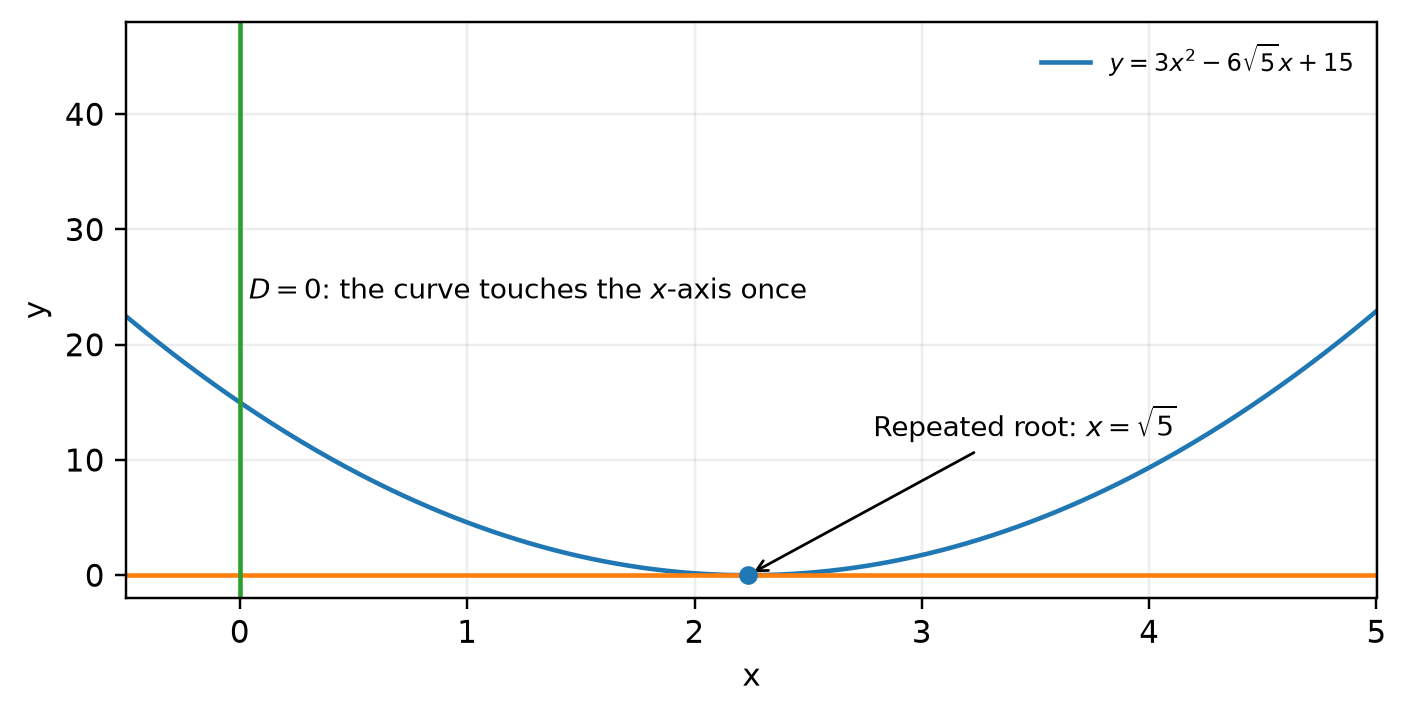
\includegraphics[width=0.92\linewidth]{figs/C10/Q01.png}\end{figure}
\par\smallskip\noindent\textbf{Code reference -}\par\noindent\fbox{\parbox{\dimexpr\linewidth-2\fboxsep-2\fboxrule\relax}{\centering\texttt{codes/C10/Q01.py}}}

\item \label{question:C10-Q03}\label{question-short:C10-Q03} Two different dice are tossed together. Find the probability that the product of their top numbers is $6$.
\engsolution
Let $X$ and $Y$ be the independent outcomes of the two fair dice. Their joint mass function is
\formulaused{P(X=i,Y=j)=P(X=i)P(Y=j)}{C10-Q03-F01}
\formulausedplain{=\frac1{36},\qquad 1\le i,j\le6.}
The product is a discrete push-forward random variable. Its probability is therefore obtained by summing the joint mass over the product preimage:
\formulaused{P(XY=z)=\sum_{ij=z}P(X=i,Y=j).}{C10-Q03}
For $z=6$, the admissible ordered pairs are
\formulausedplain{
\{(i,j):ij=6\}=\{(1,6),(2,3),(3,2),(6,1)\}.
}
There are four equally likely pairs out of $6\times6=36$, so
\formulausedplain{
P(XY=6)=4\left(\frac1{36}\right)=\frac4{36}=\frac19.
}
The four pairs exhaust the positive factorisations of $6$ within the die support, which verifies that no outcome has been omitted.
\begin{figure}[H]\centering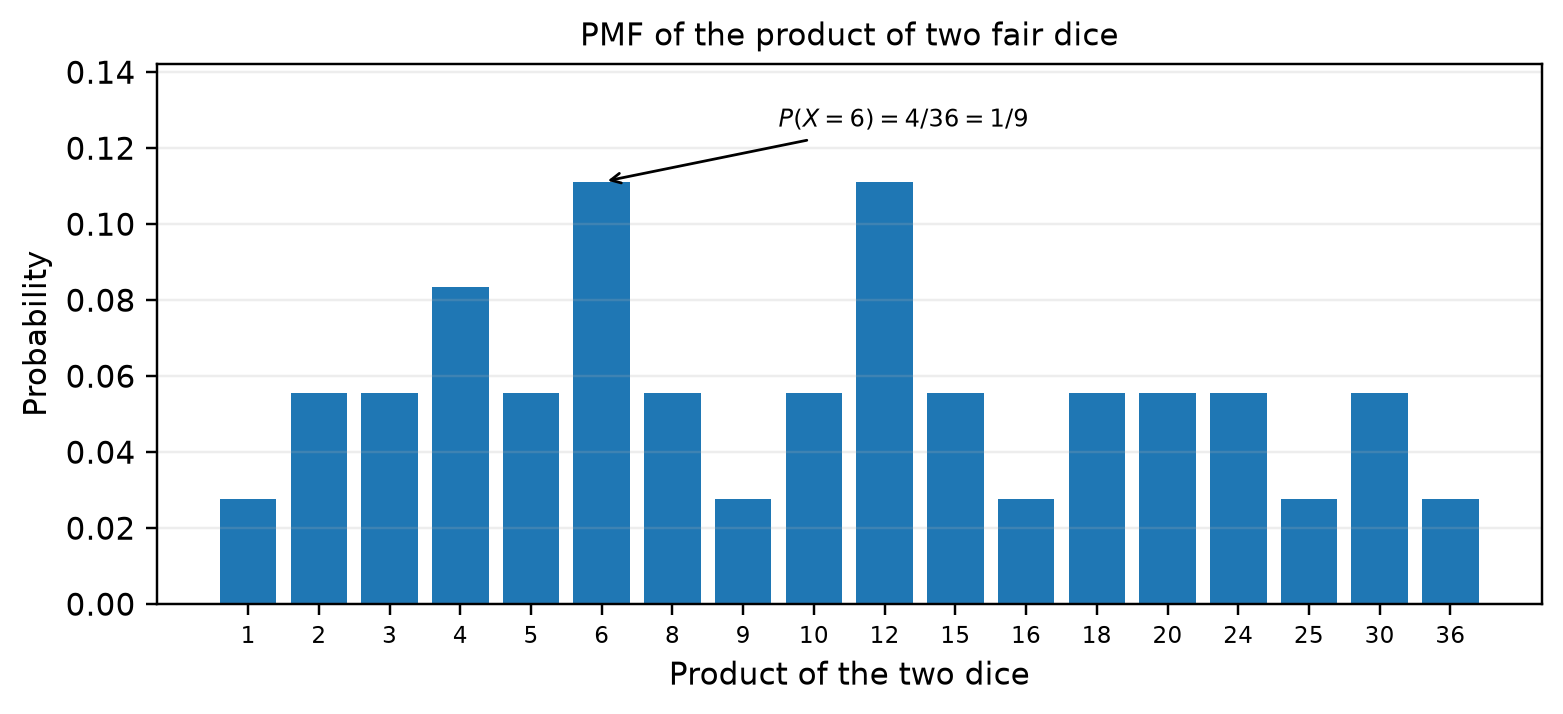
\includegraphics[width=0.98\linewidth]{figs/C10/Q03.png}\end{figure}
\par\smallskip\noindent\textbf{Code reference -}\par\noindent\fbox{\parbox{\dimexpr\linewidth-2\fboxsep-2\fboxrule\relax}{\centering\texttt{codes/C10/Q03.py}}}

\item \label{question:C10-Q08}\label{question-short:C10-Q08} In an arithmetic progression, $S_5+S_7=167$ and $S_{10}=235$. Find the AP.
\engsolution
For an AP with first term $a$ and common difference $d$,
\formulaused{
S_n=\frac n2\bigl(2a+(n-1)d\bigr).
}{C10-Q08-F01}
Consequently,
\formulausedplain{S_5+S_7=(5a+10d)+(7a+21d)=12a+31d.}
\formulausedplain{S_{10}=10a+45d.}
Writing $u=(a,d)^T$, the engineering linear-system model is
\formulaused{Au=b.}{C10-Q08}
\formulausedplain{A=\myvec{12&31\\10&45}.}
\formulausedplain{b=\myvec{167\\235}.}
Use the Jacobi splitting $A=D+L+U$, where
\formulausedplain{D=\myvec{12&0\\0&45}.}
\formulausedplain{L+U=\myvec{0&31\\10&0}.}
The iteration and its matrix are
\formulaused{u^{(k+1)}=D^{-1}\bigl[b-(L+U)u^{(k)}\bigr].}{C10-Q08-F04}
\formulaused{B=-D^{-1}(L+U)}{C10-Q08-F04-S01}
\formulausedplain{=\myvec{0&-31/12\\-2/9&0}.}
Since $\rho(B)=\sqrt{31/54}<1$, the iteration converges to the unique fixed point. Solving the fixed-point equations gives
\formulausedplain{12a+31d=167.}
\formulausedplain{10a+45d=235.}
and elimination yields $115d=575$, so $d=5$ and then $a=1$. Hence
\formulausedplain{
1,6,11,16,\ldots.
}
Finally, $S_5=5+10(5)=55$ and $S_7=7+21(5)=112$, while $S_{10}=10+45(5)=235$. The residual vector is therefore $(0,0)^T$.
\par\smallskip\noindent\textbf{Code reference -}\par\noindent\fbox{\parbox{\dimexpr\linewidth-2\fboxsep-2\fboxrule\relax}{\centering\texttt{codes/C10/Q08.py}}}

\item \label{question:C10-Q10}\label{question-short:C10-Q10} If $A(x,y)$, $B(-5,7)$ and $C(-4,5)$ are collinear, find the relation between $x$ and $y$.
\engsolution
Collinearity means that the two displacement vectors from $A$ are linearly dependent. Their determinant must therefore vanish:
\formulausedplain{\det\myvec{-5-x&7-y\\-4-x&5-y}=0.}
Subtracting the first row from the second gives the equivalent translated determinant
\formulausedplain{
\det\myvec{x+5&y-7\\1&-2}=0.
}
Expanding along the first row,
\formulausedplain{
-2(x+5)-(y-7)=0
\Longrightarrow -2x-y-3=0.
}
Thus the required rank-deficiency relation is
\formulausedplain{
2x+y+3=0.
}

\item \label{question:C10-Q11}\label{question-short:C10-Q11} The 14th term of an AP is twice its 8th term. If the 6th term is $-8$, find the sum of its first 20 terms.
\engsolution
Model the AP as the discrete-time sequence $x[n]=a+(n-1)d$, $n\ge1$. Its unilateral transform separates the constant and ramp components:
\formulaused{X(z)=\sum_{n=1}^{\infty}x[n]z^{-n}=\frac{az^{-1}}{1-z^{-1}}+\frac{dz^{-1}}{(1-z^{-1})^2}.}{C10-Q11}
The term conditions give two linear equations:
\formulausedplain{
a+13d=2(a+7d),\qquad a+5d=-8.
}
The first equation reduces to $a+d=0$, so $a=-d$. Substitution into the second equation gives
\formulausedplain{a+13d=2(a+7d).}
\formulausedplain{a+5d=-8.}
The twentieth partial sum is consequently
\formulausedplain{
S_{20}=\frac{20}{2}\bigl(2a+19d\bigr)=10(4-38)=-340.
}
The sequence generated by $(a,d)=(2,-2)$ has $t_6=-8$ and $t_{14}=-24=2t_8$, confirming both data constraints.
\par\smallskip\noindent\textbf{Code reference -}\par\noindent\fbox{\parbox{\dimexpr\linewidth-2\fboxsep-2\fboxrule\relax}{\centering\texttt{codes/C10/Q11.py}}}

\item \label{question:C10-Q15}\label{question-short:C10-Q15} A jar contains only red, blue and orange balls. The probabilities of drawing a red and a blue ball are $\frac14$ and $\frac13$, respectively. If there are 10 orange balls, find the total number of balls.
\engsolution
Let $N$ be the total number of balls. The red, blue, and orange counts must be nonnegative integers, and probability conservation gives
\formulaused{P(R)+P(B)+P(O)=1.}{C10-Q15}
\formulausedplain{\frac14+\frac13+\frac{10}{N}=1.}
Combining the first two fractions,
\formulausedplain{\frac14+\frac13=\frac7{12}.}
\formulausedplain{\frac{10}{N}=1-\frac7{12}=\frac5{12}.}
Therefore $N=10(12/5)=24$. The implied counts are
\formulausedplain{
R=\frac N4=6,\qquad B=\frac N3=8,\qquad O=10,
}
and $R+B+O=6+8+10=24$. Thus the integer feasibility check agrees with
\formulausedplain{
N=24.
}
\begin{figure}[H]\centering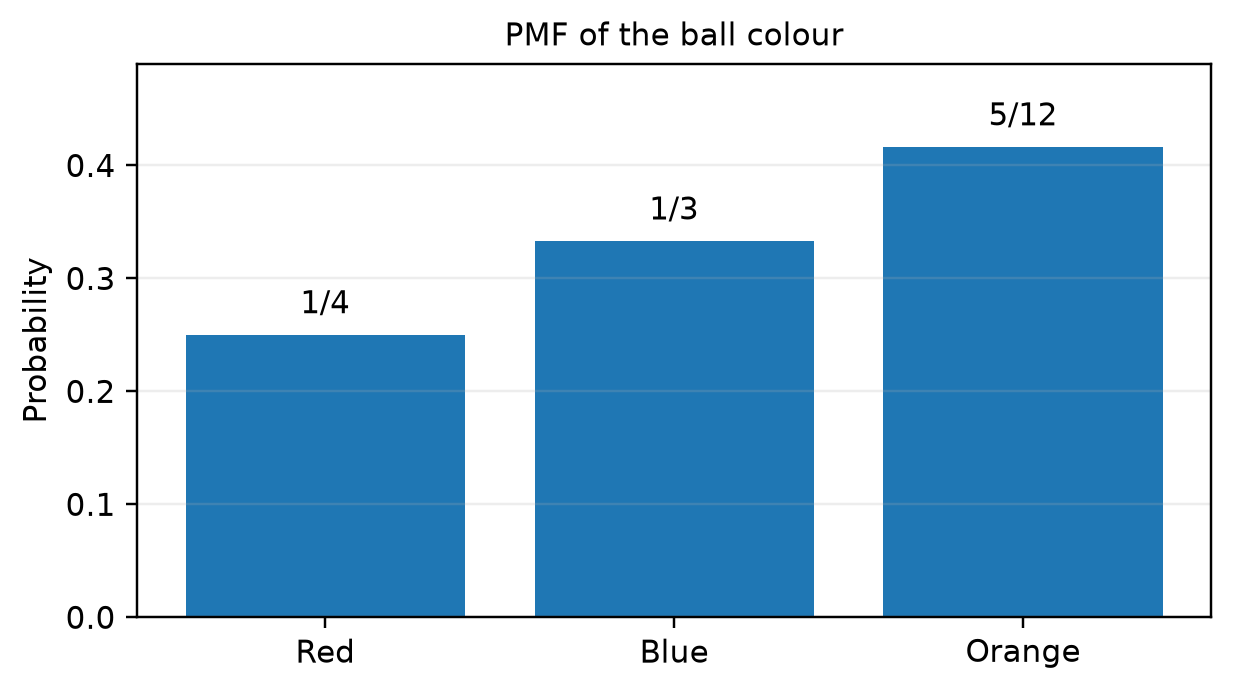
\includegraphics[width=0.9\linewidth]{figs/C10/Q15.png}\end{figure}
\par\smallskip\noindent\textbf{Code reference -}\par\noindent\fbox{\parbox{\dimexpr\linewidth-2\fboxsep-2\fboxrule\relax}{\centering\texttt{codes/C10/Q15.py}}}

\item \label{question:C10-Q22}\label{question-short:C10-Q22} Find the 60th term of the AP $8,10,12,\ldots$ and the sum of its last 10 terms.
\engsolution
Index the finite AP from zero so that $x[n]=8+2n$ for $0\le n\le59$. The finite-support signal, rather than an infinite extension, is represented by
\formulausedplain{X(z)=8\sum_{n=0}^{59}z^{-n}+2\sum_{n=0}^{59}nz^{-n}.}
The requested term is the sample at the final index:
\formulausedplain{
x[59]=8+2(59)=126.
}
The last ten terms are indexed by $n=50,\ldots,59$, with
\formulausedplain{x[50]=8+100=108.}
\formulausedplain{x[59]=126.}
Using the arithmetic-series sum,
\formulausedplain{
\sum_{n=50}^{59}x[n]=\frac{10}{2}(108+126)=5(234)=1170.
}
The finite index range confirms that no samples beyond the 60-term support have entered the calculation.
\par\smallskip\noindent\textbf{Code reference -}\par\noindent\fbox{\parbox{\dimexpr\linewidth-2\fboxsep-2\fboxrule\relax}{\centering\texttt{codes/C10/Q22.py}}}

\item \label{question:C10-Q28}\label{question-short:C10-Q28} A card is drawn from a well-shuffled 52-card deck. Find the probability that it is (i) a spade or an ace, (ii) a black king, (iii) neither a jack nor a king, (iv) either a king or a queen.
\engsolution
Use indicator variables to preserve the overlap correction in unions. For a spade $S$ and an ace $A$, $|S|=13$, $|A|=4$, and $|S\cap A|=1$. Thus
\formulaused{\mathbf 1_{S\cup A}=\mathbf 1_S+\mathbf 1_A-\mathbf 1_{S\cap A}.}{C10-Q28}
\formulausedplain{P(S\cup A)=\frac{|S|+|A|-|S\cap A|}{52}.}
The four requested probabilities follow from the corresponding event counts:
\formulausedplain{P(S\cup A)=\frac{13+4-1}{52}=\frac4{13}.}
\formulausedplain{P(\text{black king})=\frac2{52}=\frac1{26}.}
\formulausedplain{
P(\text{neither jack nor king})=1-\frac{4+4}{52}=\frac{44}{52}=\frac{11}{13},
}
and, since kings and queens are disjoint,
\formulausedplain{
P(K\cup Q)=\frac{4+4}{52}=\frac2{13}.
}
Hence the answers are
\formulausedplain{
\frac4{13},\quad \frac1{26},\quad \frac{11}{13},\quad \frac2{13}.
}

\item \label{question:C10-Q29}\label{question-short:C10-Q29} Find $k$ if the triangle with vertices $(1,-1)$, $(-4,2k)$ and $(-k,-5)$ has area 24 square units.
\engsolution
The determinant of the two edge vectors gives twice the signed area. With $A=(1,-1)$, $B=(-4,2k)$, and $C=(-k,-5)$,
\formulaused{2[ABC]=\left|\det(B-A,C-A)\right|}{C10-Q29}
\formulausedplain{=\left|\det\myvec{-5&2k+1\\-k-1&-4}\right|=|2k^2+3k+21|.}
The inner quadratic is always positive because its discriminant is $3^2-4(2)(21)=-159<0$ and its leading coefficient is positive. Therefore the absolute value can be removed, and the area condition becomes
\formulausedplain{
2k^2+3k+21=48\Longrightarrow 2k^2+3k-27=0.
}
Applying the quadratic formula,
\formulausedplain{
k=\frac{-3\pm\sqrt{9+216}}4=\frac{-3\pm15}{4}.
}
Thus both feasible parameter values are
\formulausedplain{
k=3\quad\text{or}\quad k=-\frac92.
}
Each value gives determinant magnitude $48$, hence area $24$.
\begin{figure}[H]\centering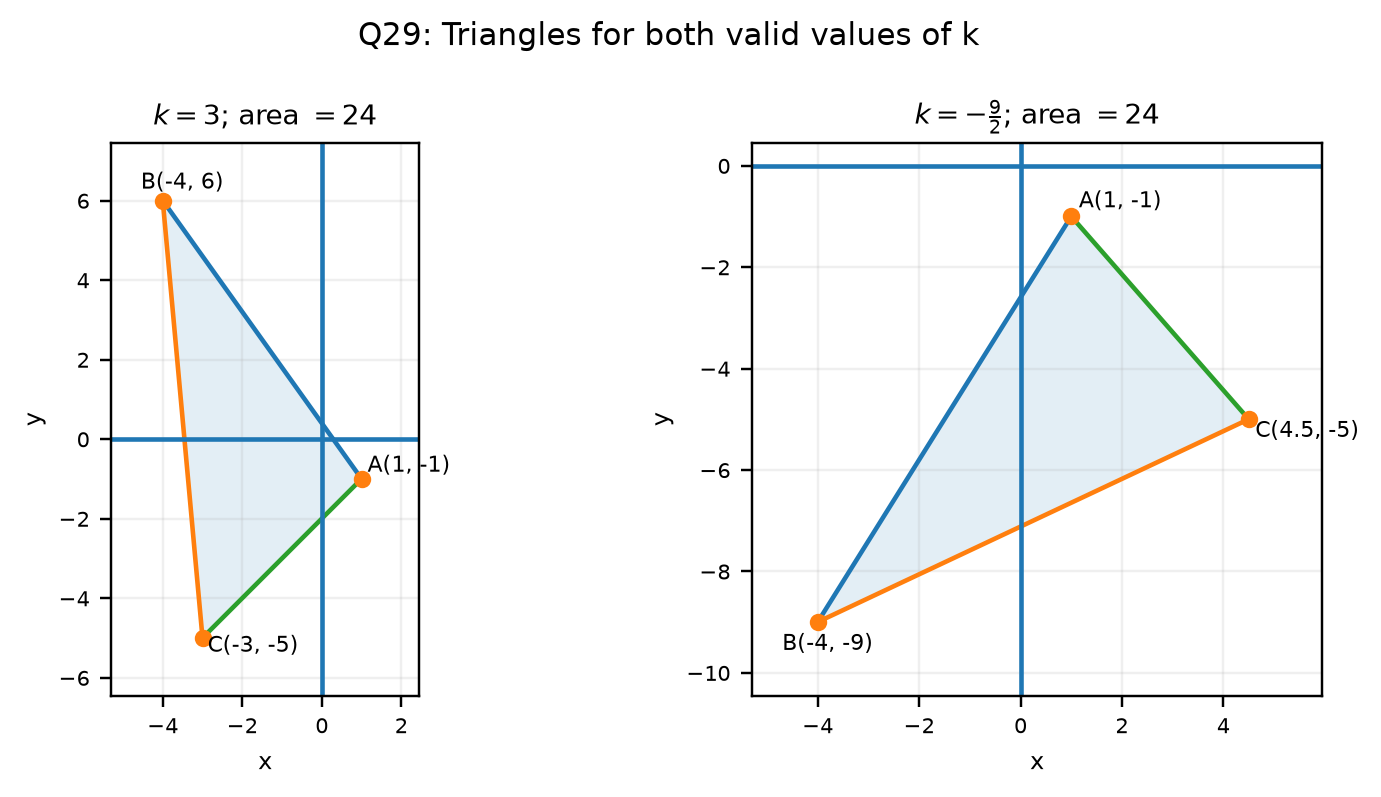
\includegraphics[width=0.99\linewidth]{figs/C10/Q29.png}\end{figure}
\par\smallskip\noindent\textbf{Code reference -}\par\noindent\fbox{\parbox{\dimexpr\linewidth-2\fboxsep-2\fboxrule\relax}{\centering\texttt{codes/C10/Q29.py}}}
\end{enumerate}


